\documentclass[11pt,a4paper]{article}

\usepackage[utf8]{inputenc}
\usepackage[T1]{fontenc}
\usepackage{amsmath,amssymb,amsfonts}
\usepackage{graphicx}
\usepackage{booktabs}
\usepackage{float}
\usepackage{hyperref}
\usepackage{xcolor}
\usepackage[margin=1in]{geometry}

\hypersetup{
    colorlinks=true,
    linkcolor=blue,
    citecolor=blue,
    urlcolor=blue
}

\newcommand{\nrmse}{\mathrm{NRMSE}}

% every inline number below is generated from the result records by make_tables.py
% generated by make_tables.py; do not edit
\newcommand{\gainQrcWindowXxz}{0.244}
\newcommand{\gainRfWindowXxz}{0.078}
\newcommand{\gainQrcWindowIsing}{0.203}
\newcommand{\gainRfWindowIsing}{0.078}
\newcommand{\gainQrcRecurrentXxz}{0.101}
\newcommand{\gainRfRecurrentXxz}{0.084}
\newcommand{\gainEsnRecurrentXxz}{0.081}
\newcommand{\gainQrcRecurrentIsing}{0.114}
\newcommand{\gainRfRecurrentIsing}{0.084}
\newcommand{\gainEsnRecurrentIsing}{0.081}
\newcommand{\exactQrcWindow}{0.632}
\newcommand{\shotsQrcWindow}{0.651}
\newcommand{\shotLossWindow}{0.019}
\newcommand{\exactWinsRfWindow}{0}
\newcommand{\exactClusterWinsRfWindow}{0}
\newcommand{\exactPRfWindow}{2.2\times10^{-6}}
\newcommand{\exactRfScaleLowWindow}{0.05}
\newcommand{\exactRfBiasHighWindow}{3}
\newcommand{\exactQrcRecurrent}{0.412}
\newcommand{\shotsQrcRecurrent}{0.523}
\newcommand{\shotLossRecurrent}{0.110}
\newcommand{\exactWinsRfRecurrent}{17}
\newcommand{\exactClusterWinsRfRecurrent}{4}
\newcommand{\exactPRfRecurrent}{0.434}
\newcommand{\exactRfScaleLowRecurrent}{0.001}
\newcommand{\exactRfBiasHighRecurrent}{10}
\newcommand{\flatQrc}{37}
\newcommand{\tpeTrialsQrc}{197}
\newcommand{\spsaEvalsQrc}{50}
\newcommand{\flatRf}{70}
\newcommand{\tpeTrialsRf}{239}
\newcommand{\spsaEvalsRf}{36}
\newcommand{\flatPoly}{99}
\newcommand{\tpeTrialsPoly}{81}
\newcommand{\spsaEvalsPoly}{12}
\newcommand{\flatLin}{100}
\newcommand{\tpeTrialsLin}{111}
\newcommand{\spsaEvalsLin}{12}
\newcommand{\maxQrcRunWinsRf}{0}
\newcommand{\maxQrcSeedWinsRf}{0}
\newcommand{\maxPRf}{2.3\times10^{-4}}
\newcommand{\minGapRf}{0.045}
\newcommand{\maxGapRf}{0.249}
\newcommand{\bestQrc}{0.369}
\newcommand{\bestPoly}{0.373}
\newcommand{\bestRf}{0.324}
\newcommand{\bestPolyRunWins}{14}
\newcommand{\bestPolyRunLosses}{10}
\newcommand{\bestPolyTies}{1}
\newcommand{\bestPolySeedWins}{4}
\newcommand{\bestPolyP}{0.157}
\newcommand{\bestPolyCiLo}{-0.0090}
\newcommand{\bestPolyCiHi}{0.0001}
\newcommand{\minGapEsn}{0.156}
\newcommand{\maxGapEsn}{0.188}
\newcommand{\esnZZ}{0.340}
\newcommand{\esnZX}{0.259}
\newcommand{\vWinIsingZX}{9.65}
\newcommand{\vRecIsingZX}{9.66}
\newcommand{\WRecXxzZX}{9.95}
\newcommand{\vHigh}{10}
\newcommand{\WHigh}{10}
\newcommand{\esnSrMax}{0.052}
\newcommand{\esnSrLow}{0.05}
\newcommand{\esnBiasMin}{9.80}
\newcommand{\esnBiasHigh}{10}
\newcommand{\kfbMin}{0.73}
\newcommand{\kfbMax}{4.77}
\newcommand{\shots}{12288}
\newcommand{\shotsPerBasisZX}{6144}
\newcommand{\nQubits}{12}
\newcommand{\widthZZ}{78}
\newcommand{\widthZX}{156}
\newcommand{\widthPoly}{90}
\newcommand{\widthLin}{12}
\newcommand{\recSteps}{3000}
\newcommand{\replayDrives}{4.5\times10^{6}}
\newcommand{\noBiasEsn}{0.445}
\newcommand{\noBiasQrc}{0.412}
\newcommand{\noBiasQrcWins}{23}
\newcommand{\biasEsn}{0.340}
\newcommand{\vTwoQrcStudySeconds}{0.14}
\newcommand{\noBiasQrcStudyHours}{3.31}
\newcommand{\gapRfWindowXxzZZ}{0.249}
\newcommand{\gapRfWindowXxzZX}{0.083}
\newcommand{\gapRfWindowIsingZZ}{0.170}
\newcommand{\gapRfWindowIsingZX}{0.045}
\newcommand{\gapRfRecurrentXxzZZ}{0.107}
\newcommand{\gapRfRecurrentXxzZX}{0.089}
\newcommand{\gapRfRecurrentIsingZZ}{0.112}
\newcommand{\gapRfRecurrentIsingZX}{0.082}
\newcommand{\ratioWinMin}{2.6}
\newcommand{\ratioWinMax}{3.1}
\newcommand{\ratioRecMin}{74}
\newcommand{\ratioRecMax}{83}
\newcommand{\qrcSdMin}{0.009}
\newcommand{\qrcSdMax}{0.018}
\newcommand{\exactRfWindow}{0.406}
\newcommand{\shotsRfWindow}{0.402}
\newcommand{\trialsMinQrc}{121}
\newcommand{\trialsMaxQrc}{197}
\newcommand{\trialsMinRf}{97}
\newcommand{\trialsMaxRf}{239}
\newcommand{\trialsMinEsn}{189}
\newcommand{\trialsMaxEsn}{279}
\newcommand{\totalHours}{22.1}
\newcommand{\gpu}{RTX 2050}
\newcommand{\nTests}{28}
\newcommand{\bonfRf}{3.2\times10^{-3}}
\newcommand{\polyWeakPLo}{0.011}
\newcommand{\polyWeakPHi}{0.023}
\newcommand{\alphaLow}{10^{-6}}
\newcommand{\alphaEdgeMax}{1.28\times10^{-6}}
\newcommand{\esnLeakMin}{0.84}
\newcommand{\esnLeakMax}{0.88}
\newcommand{\esnKeepMin}{0.12}
\newcommand{\esnKeepMax}{0.16}
\newcommand{\gapShrinkRecMin}{0.02}
\newcommand{\gapShrinkRecMax}{0.03}
\newcommand{\persMin}{1.13}
\newcommand{\persMax}{1.16}
\newcommand{\exactCommitWindow}{4538057}
\newcommand{\shotsCommitWindow}{a902b04}
\newcommand{\exactCommitRecurrent}{4538057}
\newcommand{\shotsCommitRecurrent}{a902b04}
\newcommand{\vptTieLinXxzWins}{12}
\newcommand{\vptTieLinXxzSeeds}{2}
\newcommand{\vptTieLinXxzP}{0.597}
\newcommand{\vptTieLinIsingWins}{19}
\newcommand{\vptTieLinIsingSeeds}{5}
\newcommand{\vptTieLinIsingP}{0.076}
\newcommand{\vptTiePolyXxzWins}{10}
\newcommand{\vptTiePolyXxzSeeds}{1}
\newcommand{\vptTiePolyXxzP}{0.937}
\newcommand{\vptTiePolyIsingWins}{12}
\newcommand{\vptTiePolyIsingSeeds}{3}
\newcommand{\vptTiePolyIsingP}{0.796}
\newcommand{\lyapExp}{0.973}
\newcommand{\lyapTimeSteps}{4.11}
\newcommand{\sampleLt}{0.24}
\newcommand{\horizonLt}{10}
\newcommand{\horizonSteps}{41}
\newcommand{\nStarts}{20}
\newcommand{\vptThreshold}{0.5}
\newcommand{\sampleEvery}{25}
\newcommand{\vptBest}{0.80}
\newcommand{\vptMaxRun}{1.08}
\newcommand{\vptPRfZXWindowLo}{0.020}
\newcommand{\vptPRfZXWindowHi}{0.035}
\newcommand{\vptPRfZZWindowLo}{2.8\times10^{-4}}
\newcommand{\vptPRfZZWindowHi}{3.5\times10^{-4}}
\newcommand{\vptPPolyZZWindowLo}{3.5\times10^{-4}}
\newcommand{\vptPPolyZZWindowHi}{8.5\times10^{-4}}
\newcommand{\polyNrmseOneLtWindow}{8.3\times10^{4}}
\newcommand{\vptPRfZXRecurrentLo}{6.8\times10^{-3}}
\newcommand{\vptPRfZXRecurrentHi}{9.5\times10^{-3}}
\newcommand{\vptPRfZZRecurrentLo}{0.082}
\newcommand{\vptPRfZZRecurrentHi}{0.153}
\newcommand{\vptPPolyZZRecurrentLo}{0.796}
\newcommand{\vptPPolyZZRecurrentHi}{0.937}
\newcommand{\polyNrmseOneLtRecurrent}{1.3\times10^{5}}
\newcommand{\vptSigRfCells}{6}
\newcommand{\vptRecZZRfSeedWinsMax}{1}
\newcommand{\vptLinMax}{0.08}
\newcommand{\vptQrcWinZZMin}{0.08}
\newcommand{\vptQrcWinZZMax}{0.13}
\newcommand{\freerunCommit}{df03eeb}
\newcommand{\freerunHours}{0.66}


\title{Finite-Shot Quantum Reservoir Computing on Lorenz-96\\
Against Tuned Classical Baselines}

\author{
    Tushar Pandey\\
    \textit{Texas A\&M University}
}

\date{\today}

\begin{document}

\maketitle

\begin{abstract}
Does a quantum reservoir computer (QRC) forecast a chaotic system better than a classical model
when the comparison is fair? We fix four conditions for a fair comparison: every classical
baseline is tuned with a search budget comparable to the QRC's, the classical models see the same
input window and have the same number of features, the QRC's headline number is read from a finite
number of measurement shots, and every result is a multi-seed statistic. Under these conditions we
run eight cells on one-step forecasting of a six-variable Lorenz-96 system with a
twelve-qubit reservoir: two memory schemes (reset and recurrent), two Hamiltonians (a disordered
XXZ chain and an all-to-all Ising model) and two readouts (one measurement basis or two). In all
eight cells the QRC loses to a random-feature map of the same width and window, on every one of
five fresh data seeds. The best QRC cell ties a degree-2 polynomial of the input window, and an
echo-state network of the same width wins every recurrent cell by a wide margin. Measuring a second,
non-commuting basis is the largest single gain for the QRC, but it does not close the gap. In one
XXZ, single-basis pair per memory scheme, finite shots cost the recurrent QRC far more than the reset
one, and a local refinement stage after the Bayesian search, tested in the best QRC cell, improves
no model. In free-running forecasts no model's mean valid prediction time reaches one Lyapunov time,
and the QRC stays behind the random features and the echo-state network; with one basis it falls
to a tie with the linear model (reset memory) or the polynomial (recurrent memory), and with two
bases it outlasts the polynomial, which diverges on its own output. All tables are generated from the stored result records.
\end{abstract}

\section{Introduction}

Quantum reservoir computing trains only a linear readout on the measured outputs of a fixed quantum
system driven by the input signal~\cite{fujii2017}. Because nothing quantum is trained, it is a
candidate for near-term hardware, and a number of studies report that a small quantum reservoir
forecasts chaotic or nonlinear time series better than a classical one~\cite{ahmed2024,
kobayashi2024,nguyen2026}. Whether such a result says something about the quantum system or about
the comparison depends on how the classical side was set up. In earlier work we found that two
commonly cited QRC advantages did not survive once the classical baseline received the same tuning
and capacity as the quantum model~\cite{pandey2026cartography}, and that a high-dimensional quantum
reservoir did not gain from its dimension when matched against classical models of the same
width~\cite{pandey2026qra}; a related study compared fixed-reservoir and variational quantum
models on the Lorenz-63 system~\cite{pandey2026qpinn}.

This paper asks the same question on a harder target and under stricter conditions. We call a
comparison fair when four conditions hold:
\begin{enumerate}
\item every classical baseline is tuned with a budget comparable to the QRC's, by the same search
  method, on the same tuning seeds;
\item the classical models see the same input window as the QRC, and those built to match it have
  the same number of features;
\item the QRC's headline number is computed from a finite number of measurement shots, as hardware
  would report it, not from exact expectation values;
\item every reported number is a statistic over fresh data seeds and reservoir seeds that were never
  used in tuning, with paired tests corrected for multiple comparisons.
\end{enumerate}

We run eight cells on one-step forecasting of Lorenz-96 with $K=6$ variables and a
$q=\nQubits$ qubit reservoir. The finding is plain. In all eight cells the QRC loses to a random
tanh feature map of the same width and window on every data seed (it wins \maxQrcRunWinsRf{} of 25
runs and \maxQrcSeedWinsRf{} of 5 data seeds in every cell; the largest Holm-corrected $p$ is
$\maxPRf$). The best QRC cell ties a degree-2 polynomial of the input window, and in the recurrent
cells an echo-state network (ESN) of the same width wins by $\minGapEsn$ to $\maxGapEsn$ in
$\nrmse$. Run as free-running forecasters, no model's mean valid prediction time reaches one
Lyapunov time (the ESN is longest, $\vptBest$), and the QRC still has a shorter mean VPT than the random features in
every cell (significantly in \vptSigRfCells{} of 8) and than the ESN in every recurrent cell.
Section~\ref{sec:related} sets out the patterns by which advantage claims are usually
made, Section~\ref{sec:protocol} the protocol, Section~\ref{sec:results} the results, and
Sections~\ref{sec:discussion} to~\ref{sec:repro} what would have to change for a QRC to win here,
the limits of the study, and how to reproduce it.

\section{How advantage claims are usually made}
\label{sec:related}

We list six patterns that recur in QRC benchmarks. None of them makes a result wrong; each makes it
answer a narrower question than an advantage claim needs. We map individual papers to the patterns
only where their own text states the relevant fact.

\paragraph{1. Resources counted in different units.} A quantum reservoir is often sized by its
number of qubits and a classical one by its number of neurons. Ahmed, Tennie and
Magri~\cite{ahmed2024} report that on Lorenz-63 their best quantum architecture at 9 to 11
qubits reaches valid prediction times similar to those of classical reservoirs of 500 to 2000
neurons (their Fig.~8). Qubits and neurons are not the
same resource for a linear readout: what the readout sees is the number of measured features. We
match that number directly.

\paragraph{2. Untuned or lightly tuned baselines.} The strength of a baseline depends on which of
its knobs are searched. Kobayashi, Fujii and Yamamoto~\cite{kobayashi2024} report the best ESN over a
grid of five spectral radii and four learning rates (their Appendix~D). Nguyen and
Soh~\cite{nguyen2026}, forecasting the Mackey-Glass series with a driven Jaynes-Cummings reservoir,
tune an ESN's spectral radius, leak, input scale and bias over 810 settings on the training loss,
while their quantum model receives grid search, Bayesian search and then a further QFI-aware
optimisation stage. Ahmed et al.~\cite{ahmed2024} tune hyperparameters with grid search and
Bayesian optimisation and find that the classical reservoir outperforms every quantum architecture
on Lorenz-63 at the same reservoir size (their Fig.~8), while three quantum architectures outperform
it on a ten-variable Lorenz-96 system as the reservoir grows (their Fig.~12). Section~\ref{sec:why}
shows in our own records how one missing knob reverses a result.

\paragraph{3. QRC compared with QRC.} Much careful work compares quantum reservoirs with each
other: across dynamical regimes~\cite{martinezpena2021} or across measurement
protocols~\cite{mujal2023}. That is the right way to design a reservoir, but a gain over another
quantum reservoir is not a gain over a classical model, and the two are easy to conflate when the
same paper uses advantage language.

\paragraph{4. Capacity metrics in place of forecast error.} Memory capacity and expressive capacity
measure what a reservoir could represent. Hu et al.~\cite{hu2023} give a framework for the expressive
capacity of a quantum system under the sampling noise of finite measurement. Capacity is useful for
design, but it does not say whether a tuned classical model forecasts the same task better.

\paragraph{5. Exact expectations in the headline, shots elsewhere.} Hardware returns counts. Ahmed
et al.~\cite{ahmed2024} report noise-free emulation and leave finite sampling to future work;
Kobayashi et al.~\cite{kobayashi2024} state their main results under negligible statistical
fluctuations and treat the statistical uncertainty of a finite number of measurements in their
Appendix~C; Nguyen and
Soh~\cite{nguyen2026} obtain their margins from expectation-value simulations and analyse finite
shots in a supplementary note. Section~\ref{sec:shots} shows that this choice can change the
verdict.

\paragraph{6. Few seeds.} A single reservoir draw on a single series gives no estimate of the
spread between draws, so a gap of a few percent cannot be told from luck. We do not attribute this
pattern to specific papers here; we report every comparison over $5\times5$ evaluation runs.

Where strong classical baselines are included, they often win: in the multivariate gate-based study
of Hamhoum et al.~\cite{hamhoum2025} the QRC matches classical reservoir computing on Lorenz-63 but a
nonlinear vector autoregression and a clustered ESN remain stronger in some settings.

\section{Protocol}
\label{sec:protocol}

All runs use the \texttt{qrc\_bench} pipeline (Section~\ref{sec:repro}). Every constant in this
section is read from the pipeline source or from the stored records.

\subsection{Task}

Lorenz-96 with $K=6$ variables on a ring, $\dot x_k = (x_{k+1}-x_{k-2})x_{k-1} - x_k + F$ with
$F=8$, is integrated by fourth-order Runge-Kutta with step $0.01$; one sample is kept every 25
steps, after 1000 discarded samples, and each variable is standardised. A series has 2000 samples
in the window cells and 3000 in the recurrent cells. The target is the next sample of all six
variables. The score is the one-step-ahead $\nrmse$ on the last 15 percent of the series, averaged
over the six variables, each normalised by its standard deviation on the test slice, so that
$\nrmse=1$ is the mean predictor. The readout is fit once on everything before the test slice,
after a washout of 50 samples (window) or 400 samples (recurrent).

\subsection{Quantum reservoir}

The reservoir has $n_{\mathrm{in}}=6$ input qubits, one per variable, and $n_{\mathrm{mem}}=6$ memory
qubits, $q=\nQubits$. Each input $x$ is angle-encoded as $R_Y(\mathrm{clip}(s\,x,-\pi,\pi))|0\rangle$
on its input qubit, with the encoding scale $s$ tuned in $[0.1,\pi]$. The system then evolves for a
time $\tau$, tuned in $[0.1,10]$, under one of two Hamiltonians, both all-to-all:
\begin{align}
H_{\mathrm{XXZ}} &= \sum_{i<j} \left(X_iX_j + Y_iY_j + \Delta\, Z_iZ_j\right) + \sum_i h_i Z_i,
  \quad h_i\sim\mathcal{U}(-W,W),\\
H_{\mathrm{Ising}} &= \sum_{i<j} J_{ij}\, X_iX_j + v\sum_i Z_i, \quad J_{ij}\sim\mathcal{U}(0,1),
\end{align}
with $\Delta\in[-2,2]$, $W\in[0.1,10]$ and $v\in[0.1,10]$ tuned. The random fields or couplings are
drawn from the reservoir seed.

\paragraph{Memory.} In the \emph{window} cells the memory is reset: at every step the memory qubits
start in $|0\rangle^{\otimes 6}$ and the last two inputs are driven in order, the input qubits being
traced out between drives. The QRC is then a fixed feature map of a two-step input window. In the
\emph{recurrent} cells the memory state is carried from step to step, one drive per step, and a
feedback term shifts every input angle by $k_{\mathrm{fb}}\tanh(\bar m_{t-1})$, where $\bar m_{t-1}$
is the mean measured $\langle Z\rangle$ of the previous step and $k_{\mathrm{fb}}\in[0,8]$ is tuned.

\paragraph{Readout.} The Z/ZZ readout measures all twelve qubits in the computational basis and
gives $\langle Z_i\rangle$ and $\langle Z_iZ_j\rangle$, $12+66=\widthZZ$ features. The Z/ZZ+X/XX
readout measures the same block a second time in the $X$ basis, giving $\widthZX$ features. The
feedback signal and the memory state stay on the $Z$ basis.

\paragraph{Shots.} Every QRC feature in the eight cells is estimated from $1024\,q=\shots$ shots per
step. With two bases the budget is split equally, $\shotsPerBasisZX$ per basis, so the second basis
costs no extra shots. We use the restarting protocol~\cite{mujal2023}: each step's measurement is a
fresh preparation of the same circuit, so the memory state carried to the next step is exact and is
never collapsed, while the features and the feedback signal are both read from the sampled counts.
The shot noise realisation is fixed by the reservoir seed. The exact-expectation runs of
Section~\ref{sec:shots} read exact values with the same protocol block, but were made with an
earlier pipeline commit (\texttt{\exactCommitWindow} against \texttt{\shotsCommitWindow}).

\subsection{Classical models}

\paragraph{Random features.} $\tanh(A z_t + b)$, where $z_t$ stacks the same two-step window the
QRC sees ($n=12$ values), $A_{ij}\sim\mathcal{N}(0,\sigma^2/n)$ and $b_i\sim\mathcal{U}(-\beta,\beta)$,
with $\sigma\in[10^{-3},10]$ and $\beta\in[0,10]$ tuned. Its width equals the QRC width in every
cell. This is the same-window, same-width control for the QRC.

\paragraph{Poly2 and linear.} The complete degree-2 polynomial of the window ($12$ linear terms and
$78$ products, width $\widthPoly$) and the window itself (width $\widthLin$). Only the ridge penalty
is tuned. Both are deterministic: they have no reservoir seed.

\paragraph{Echo-state network.} In the recurrent cells, a leaky ESN of the same width as the QRC,
$r_t=(1-a)\,r_{t-1}+a\tanh(W r_{t-1}+W_{\mathrm{in}}x_t+b)$, with spectral radius in $[0.05,1.5]$, leak
$a\in[0.01,1]$, input scale in $[0.01,5]$, density in $[0.02,1]$ and bias scale in $[0,10]$ tuned. It
sees the whole history, as the recurrent QRC does; the window models remain as references at a
two-step window. (As tuned, the ESN's memory is short; see Section~\ref{sec:results}.)

\subsection{Tuning}

Every model is tuned by Optuna's TPE sampler~\cite{akiba2019} with the same sampler seed. The ridge
penalty $\alpha$ is tuned in $[10^{-6},10^{2}]$ (log scale) for every model, on standardised
features, and counts as a knob. The budget is matched by search density rather than trial count:
a model with $d$ knobs gets at least $25d$ trials and continues until 50 trials pass without a new
best, with a cap of 300. Every model in every cell stopped on the patience rule, after
\trialsMinQrc{} to \trialsMaxQrc{} trials for the QRC, \trialsMinRf{} to \trialsMaxRf{} for the
random features and \trialsMinEsn{} to \trialsMaxEsn{} for the ESN. The objective is the
validation $\nrmse$ averaged over three rolling-origin folds (each 10 percent of the series, all
before the test slice) and over three tuning data seeds $\times$ three tuning reservoir seeds. The
best setting of each model is then frozen and evaluated once on five fresh data seeds $\times$ five
fresh reservoir seeds, which share no seed with tuning.

\subsection{Statistics}

For each QRC-versus-classical pair we form the paired difference on each of the 25 evaluation runs
and on each of the 5 data-seed clusters (the mean over that seed's five reservoir seeds). We report
how many runs and data seeds the QRC wins (a difference within $5\times10^{-4}$ counts as a tie), a
cluster bootstrap 95 percent interval (20000 resamples), and a paired $t$-test on the cluster means,
Holm-corrected over the comparisons in the cell (three in a window cell, four in a recurrent cell).
The Holm family is the cell, not the grid: the eight cells hold $\nTests$ tests in all, and no
correction across cells is applied. The random-feature verdict survives any such correction: the
largest uncorrected cluster-level $p$ against the random features, times $\nTests$, is $\bonfRf$.
The weaker Poly2 results (Holm $p=\polyWeakPLo$ and $\polyWeakPHi$ in the recurrent two-basis cells)
may not.
For Poly2 and linear the five reservoir seeds of a data seed share one classical prediction, so the
run-level tests are not independent; we flag them and use the cluster-level test throughout.

\section{Results}
\label{sec:results}

\subsection{The eight cells}

Table~\ref{tab:nrmse} gives the test $\nrmse$ of every model in every cell and
Tables~\ref{tab:stats} and~\ref{tab:statsp} the paired statistics; Fig.~\ref{fig:cells} shows the same numbers.

\begin{table}[htbp]
\centering
\caption{Test $\nrmse$ (mean $\pm$ s.d.\ over 25 evaluation runs, one-step ahead, lower is better)
in the eight cells. QRC features are read from $\shots$ shots per step. Width is the QRC width, which
the random features (RF) and the ESN match; readout ``+X/XX'' is Z/ZZ plus the $X$ basis. Poly2 has
width $\widthPoly$ and linear $\widthLin$. Bold:
best model in the cell. Poly2 and linear depend only on the data, so they repeat within a memory
kind; the window and recurrent kinds use series of different length.}
\label{tab:nrmse}
\footnotesize\setlength{\tabcolsep}{3pt}\begin{tabular}{lllrccccc}
\toprule
Kind & Res. & Readout & Width & QRC & RF & Poly2 & Linear & ESN \\
\midrule
window & XXZ & Z/ZZ & 78 & $0.651\pm0.018$ & $0.402\pm0.013$ & $\mathbf{0.373}\pm0.013$ & $0.712\pm0.010$ & -- \\
window & XXZ & +X/XX & 156 & $0.407\pm0.018$ & $\mathbf{0.324}\pm0.016$ & $0.373\pm0.013$ & $0.712\pm0.010$ & -- \\
window & Ising & Z/ZZ & 78 & $0.572\pm0.013$ & $0.402\pm0.013$ & $\mathbf{0.373}\pm0.013$ & $0.712\pm0.010$ & -- \\
window & Ising & +X/XX & 156 & $0.369\pm0.012$ & $\mathbf{0.324}\pm0.016$ & $0.373\pm0.013$ & $0.712\pm0.010$ & -- \\
\midrule
recurrent & XXZ & Z/ZZ & 78 & $0.523\pm0.018$ & $0.416\pm0.016$ & $0.392\pm0.018$ & $0.716\pm0.010$ & $\mathbf{0.340}\pm0.012$ \\
recurrent & XXZ & +X/XX & 156 & $0.421\pm0.012$ & $0.332\pm0.017$ & $0.392\pm0.018$ & $0.716\pm0.010$ & $\mathbf{0.259}\pm0.017$ \\
recurrent & Ising & Z/ZZ & 78 & $0.528\pm0.012$ & $0.416\pm0.016$ & $0.392\pm0.018$ & $0.716\pm0.010$ & $\mathbf{0.340}\pm0.012$ \\
recurrent & Ising & +X/XX & 156 & $0.414\pm0.009$ & $0.332\pm0.017$ & $0.392\pm0.018$ & $0.716\pm0.010$ & $\mathbf{0.259}\pm0.017$ \\
\bottomrule
\end{tabular}

\end{table}

\begin{table}[htbp]
\centering
\caption{QRC wins against each classical model, per cell: evaluation runs (of 25) and, in
parentheses, data seeds (of 5, by cluster mean) on which the QRC has the lower test $\nrmse$.
$^\dagger$: the classical model has no reservoir seed, so run-level counts are not independent.}
\label{tab:stats}
\small
\begin{tabular}{lllcccc}
\toprule
Kind & Res. & Readout & vs Random features & vs Poly2 & vs Linear & vs ESN \\
\midrule
window & XXZ & Z/ZZ & 0/25 (0/5) & 0/25 (0/5)$^\dagger$ & 25/25 (5/5)$^\dagger$ & -- \\
window & XXZ & +X/XX & 0/25 (0/5) & 0/25 (0/5)$^\dagger$ & 25/25 (5/5)$^\dagger$ & -- \\
window & Ising & Z/ZZ & 0/25 (0/5) & 0/25 (0/5)$^\dagger$ & 25/25 (5/5)$^\dagger$ & -- \\
window & Ising & +X/XX & 0/25 (0/5) & 14/25 (4/5)$^\dagger$ & 25/25 (5/5)$^\dagger$ & -- \\
\midrule
recurrent & XXZ & Z/ZZ & 0/25 (0/5) & 0/25 (0/5)$^\dagger$ & 25/25 (5/5)$^\dagger$ & 0/25 (0/5) \\
recurrent & XXZ & +X/XX & 0/25 (0/5) & 0/25 (0/5)$^\dagger$ & 25/25 (5/5)$^\dagger$ & 0/25 (0/5) \\
recurrent & Ising & Z/ZZ & 0/25 (0/5) & 0/25 (0/5)$^\dagger$ & 25/25 (5/5)$^\dagger$ & 0/25 (0/5) \\
recurrent & Ising & +X/XX & 0/25 (0/5) & 1/25 (0/5)$^\dagger$ & 25/25 (5/5)$^\dagger$ & 0/25 (0/5) \\
\bottomrule
\end{tabular}

\end{table}

\begin{table}[htbp]
\centering
\caption{Holm-corrected $p$ of the QRC against each classical model, per cell: paired $t$-test on
the five data-seed means, Holm-corrected within the cell.}
\label{tab:statsp}
\small
\begin{tabular}{lllcccc}
\toprule
Kind & Res. & Readout & vs Random features & vs Poly2 & vs Linear & vs ESN \\
\midrule
window & XXZ & Z/ZZ & $2.7\times10^{-6}$ & $2.7\times10^{-6}$ & $1.3\times10^{-4}$ & -- \\
window & XXZ & +X/XX & $1.3\times10^{-5}$ & $6.7\times10^{-5}$ & $1.1\times10^{-7}$ & -- \\
window & Ising & Z/ZZ & $1.3\times10^{-5}$ & $1.3\times10^{-5}$ & $3.1\times10^{-5}$ & -- \\
window & Ising & +X/XX & $2.3\times10^{-4}$ & $0.157$ & $6.5\times10^{-8}$ & -- \\
\midrule
recurrent & XXZ & Z/ZZ & $7.4\times10^{-5}$ & $7.4\times10^{-5}$ & $1.2\times10^{-6}$ & $1.9\times10^{-6}$ \\
recurrent & XXZ & +X/XX & $1.1\times10^{-4}$ & $0.011$ & $2.3\times10^{-7}$ & $2.2\times10^{-5}$ \\
recurrent & Ising & Z/ZZ & $5.1\times10^{-5}$ & $5.1\times10^{-5}$ & $2.3\times10^{-7}$ & $2.3\times10^{-6}$ \\
recurrent & Ising & +X/XX & $1.4\times10^{-4}$ & $0.023$ & $1.2\times10^{-7}$ & $2.2\times10^{-5}$ \\
\bottomrule
\end{tabular}

\end{table}

\begin{figure}[htbp]
\centering
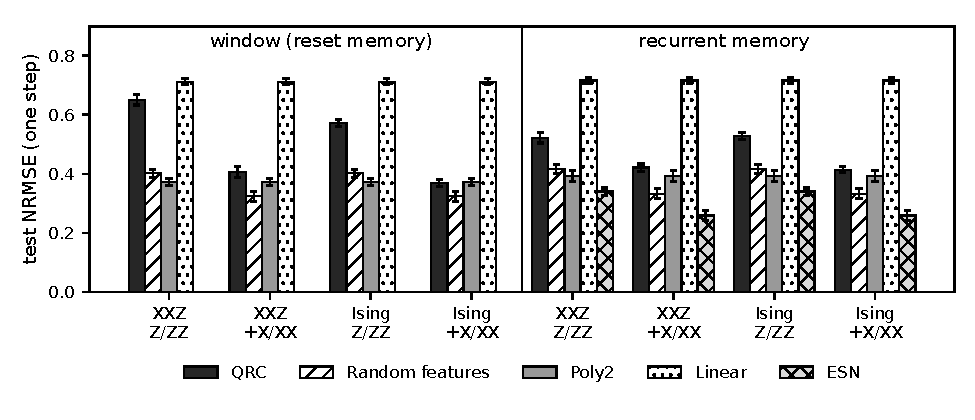
\includegraphics[width=\linewidth]{figures/fig_cells.pdf}
\caption{Test $\nrmse$ per model in the eight cells (mean $\pm$ s.d.\ over 25 runs). The random
features (hatched) are below the QRC (black) in every cell; the ESN is lowest in every recurrent
cell.}
\label{fig:cells}
\end{figure}

\paragraph{Random features beat the QRC everywhere.} In every cell the width-matched random-feature
map has the lower test $\nrmse$ on all 25 runs and all 5 data seeds, by $\minGapRf$ to $\maxGapRf$,
with Holm-corrected $p\le\maxPRf$. The random features see exactly the same two-step window and have
exactly the same number of features as the QRC, so neither input nor readout width explains the gap.

\paragraph{The second basis is the QRC's largest gain, and it does not close the gap.}
Table~\ref{tab:basis} compares each Z/ZZ cell with its Z/ZZ+X/XX partner. Adding the $X$ basis
lowers the QRC's $\nrmse$ by $\gainQrcWindowXxz$ (window, XXZ), $\gainQrcWindowIsing$ (window,
Ising), $\gainQrcRecurrentXxz$ (recurrent, XXZ) and $\gainQrcRecurrentIsing$ (recurrent, Ising),
although each basis now gets half the shots. The largest of these is the largest change of the QRC
between any two cells that differ in one factor. The
width-matched classical models gain too, from the doubled width alone: the random features by
$\gainRfWindowXxz$ (window) and $\gainRfRecurrentXxz$ (recurrent), the ESN by
$\gainEsnRecurrentXxz$. In the recurrent cells the random features' gain is $\ratioRecMin$ to
$\ratioRecMax$ percent of the QRC's, so the gap shrinks only by $\gapShrinkRecMin$ to
$\gapShrinkRecMax$ (recurrent Ising: $\gapRfRecurrentIsingZZ$ to $\gapRfRecurrentIsingZX$). In the window cells the QRC gains
$\ratioWinMin$ to $\ratioWinMax$ times as much as the random features, and the gap to them shrinks
from $\gapRfWindowXxzZZ$ (XXZ) and $\gapRfWindowIsingZZ$ (Ising) to $\gapRfWindowXxzZX$ and
$\gapRfWindowIsingZX$ (last two columns of Table~\ref{tab:basis}), but the QRC still loses on every
seed.

\begin{table}[htbp]
\centering
\caption{Effect of the second measurement basis. Columns 3 and 4: QRC test $\nrmse$ with one and
two bases (width $\widthZZ$ and $\widthZX$, same total shots). Columns 5 to 7: change in mean test
$\nrmse$ from Z/ZZ to Z/ZZ+X/XX for the QRC and for the width-matched random features (RF) and ESN,
whose width doubles with the QRC's. Columns 8 and 9: QRC minus random-feature $\nrmse$.}
\label{tab:basis}
\small
\begin{tabular}{llccccccc}
\toprule
 & & \multicolumn{2}{c}{QRC NRMSE} & \multicolumn{3}{c}{change Z/ZZ $\to$ +X/XX} & \multicolumn{2}{c}{QRC $-$ RF} \\
\cmidrule(lr){3-4}\cmidrule(lr){5-7}\cmidrule(lr){8-9}
Kind & Res. & Z/ZZ & +X/XX & QRC & RF & ESN & Z/ZZ & +X/XX \\
\midrule
window & XXZ & 0.651 & 0.407 & $-0.244$ & $-0.078$ & -- & 0.249 & 0.083 \\
window & Ising & 0.572 & 0.369 & $-0.203$ & $-0.078$ & -- & 0.170 & 0.045 \\
recurrent & XXZ & 0.523 & 0.421 & $-0.101$ & $-0.084$ & $-0.081$ & 0.107 & 0.089 \\
recurrent & Ising & 0.528 & 0.414 & $-0.114$ & $-0.084$ & $-0.081$ & 0.112 & 0.082 \\
\bottomrule
\end{tabular}

\end{table}

\paragraph{The best QRC ties Poly2.} The best QRC cell (window, Ising, Z/ZZ+X/XX) reaches
$\bestQrc$ against Poly2's $\bestPoly$. It wins \bestPolyRunWins{} of 25 runs, loses
\bestPolyRunLosses{} and ties \bestPolyTies, and wins \bestPolySeedWins{} of 5 data seeds, but the
cluster interval of the difference, $[\bestPolyCiLo,\bestPolyCiHi]$, contains zero and the Holm $p$
is $\bestPolyP$: a tie. The random features in the same cell reach $\bestRf$. In every other cell
Poly2 beats the QRC. Every QRC beats the linear model on every run.

\paragraph{The ESN wins the recurrent kind by a wide margin.} In the four recurrent cells the ESN of
the same width is ahead of the recurrent QRC on every run and every data seed, by $\minGapEsn$ to
$\maxGapEsn$ in $\nrmse$ (Tables~\ref{tab:stats} and~\ref{tab:statsp}). The ESN at width $\widthZX$ ($\esnZX$) is the best
model in the whole grid. Its history is long only in name: as tuned, the spectral radius is about
$\esnSrLow$ and the leak $\esnLeakMin$ to $\esnLeakMax$, so the state keeps a weight of only
$\esnKeepMin$ to $\esnKeepMax$ on its previous value plus a weak recurrent term, and the past fades
within a few steps. The recurrent QRC is not better than the reset QRC with two bases either.

\subsection{Shot noise}
\label{sec:shots}

Table~\ref{tab:shots} and Fig.~\ref{fig:shots} compare the XXZ, Z/ZZ cells with runs that read exact
expectation values under the same protocol block but an earlier pipeline commit
(\texttt{\exactCommitWindow} against \texttt{\shotsCommitWindow}); in both conditions the QRC is tuned under the
condition it is evaluated in. The reset QRC loses $\shotLossWindow$ in $\nrmse$ to the shots
($\exactQrcWindow\to\shotsQrcWindow$), the recurrent QRC $\shotLossRecurrent$
($\exactQrcRecurrent\to\shotsQrcRecurrent$). The difference is consistent with the role of feedback:
in the recurrent cells the feedback signal is read from the sampled counts, so measurement noise
enters the drive and is carried forward in the memory state, while in the reset cells it touches
only the readout. We have not run the ablation that separates the two (sampled readout with exact
feedback), so this is the likely mechanism, not a measured one.

The shots change the verdict, not only the number. With exact expectations the recurrent QRC
\emph{ties} the random features: it wins \exactWinsRfRecurrent{} of 25 runs and
\exactClusterWinsRfRecurrent{} of 5 data seeds, Holm $p=\exactPRfRecurrent$. With $\shots$ shots it
loses to them on every run. A study that reported exact values would have found parity with a
tuned, width-matched classical model where hardware would find a loss.

The classical models do not use shots. In the recurrent pair their rows are identical. In the
window pair Poly2 and linear are identical; the random features differ ($\exactRfWindow$ against $\shotsRfWindow$)
because the exact run was made with an earlier pipeline version that searched a narrower
random-feature range (scale $\ge\exactRfScaleLowWindow$, bias scale $\le\exactRfBiasHighWindow$).

\begin{table}[htbp]
\centering
\caption{Exact expectation values against $\shots$ shots per step, XXZ reservoir, Z/ZZ readout. Mean
test $\nrmse$ over 25 runs; ``change'' is shots minus exact. In the window pair the random features
of the exact run were tuned over a narrower range (see text).}
\label{tab:shots}
\small
\begin{tabular}{lcccccc}
\toprule
 & \multicolumn{3}{c}{window, XXZ, Z/ZZ} & \multicolumn{3}{c}{recurrent, XXZ, Z/ZZ} \\
\cmidrule(lr){2-4}\cmidrule(lr){5-7}
Model & exact & 12288 shots & change & exact & 12288 shots & change \\
\midrule
QRC & 0.632 & 0.651 & $+0.019$ & 0.412 & 0.523 & $+0.110$ \\
Random features & 0.406 & 0.402 & $-0.004$ & 0.416 & 0.416 & $0$ \\
Poly2 & 0.373 & 0.373 & $0$ & 0.392 & 0.392 & $0$ \\
Linear & 0.712 & 0.712 & $0$ & 0.716 & 0.716 & $0$ \\
ESN & -- & -- & -- & 0.340 & 0.340 & $0$ \\
\bottomrule
\end{tabular}

\end{table}

\begin{figure}[htbp]
\centering
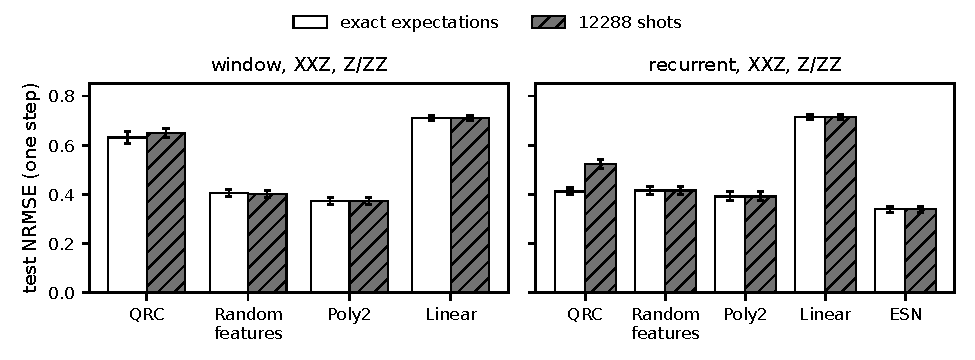
\includegraphics[width=\linewidth]{figures/fig_shots.pdf}
\caption{Exact expectation values (white) against $\shots$ shots per step (hatched), XXZ reservoir,
Z/ZZ readout (mean $\pm$ s.d.\ over 25 runs). Only the QRC changes, and the recurrent QRC changes
most.}
\label{fig:shots}
\end{figure}

\subsection{Is the search finished? A local refinement stage}
\label{sec:refine}

A tuned comparison is only as good as its search. To test whether TPE had stopped short, we
repeated the best QRC cell (window, Ising, Z/ZZ+X/XX) with a refinement stage: after TPE stops, SPSA
runs from the best TPE trial in the unit cube of each model's search space, with half the model's
floor budget, rounded down to an even number, in further evaluations, for every model. The TPE stage of this run reproduced the
original run trial for trial, so the refinement starts from the same point.

The refinement improved no model: the gain is $0$ for all four (Table~\ref{tab:refine},
Fig.~\ref{fig:conv}). The landscapes near the optimum are flat for the classical models:
\flatRf{} percent of the random features' TPE trials, \flatPoly{} percent of Poly2's and \flatLin{}
percent of the linear model's lie within $0.02$ of their best validation $\nrmse$. The QRC's landscape
is rougher, with \flatQrc{} percent of its trials within $0.02$, but a local search from its best
point finds nothing either. Since the frozen settings did not change, the test results of this run
are identical to those of the cell in Table~\ref{tab:nrmse}.

\begin{table}[htbp]
\centering
\caption{SPSA refinement after TPE, window, Ising, Z/ZZ+X/XX. Knobs include the ridge penalty.
Validation $\nrmse$ is the tuning objective. ``within 0.02'': fraction of TPE trials whose
validation $\nrmse$ is within $0.02$ of the best TPE trial.}
\label{tab:refine}
\footnotesize\setlength{\tabcolsep}{3pt}\begin{tabular}{lccccccc}
\toprule
Model & knobs & TPE trials & SPSA evals & best TPE val. & best SPSA val. & gain & within 0.02 \\
\midrule
QRC & 4 & 197 & 50 & 0.3845 & 0.3852 & 0.0 & 37\% \\
Random features & 3 & 239 & 36 & 0.3570 & 0.3586 & 0.0 & 70\% \\
Poly2 & 1 & 81 & 12 & 0.4069 & 0.4070 & 0.0 & 99\% \\
Linear & 1 & 111 & 12 & 0.7246 & 0.7246 & 0.0 & 100\% \\
\bottomrule
\end{tabular}

\end{table}

\begin{figure}[htbp]
\centering
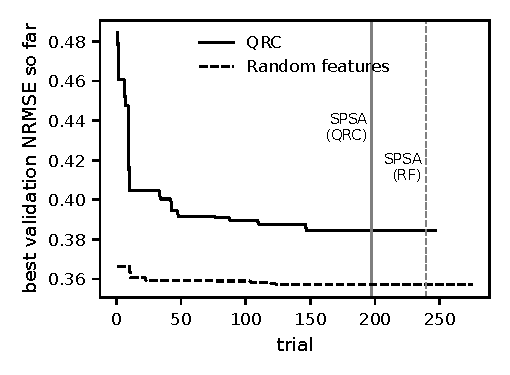
\includegraphics[width=0.6\linewidth]{figures/fig_convergence.pdf}
\caption{Best validation $\nrmse$ so far against trial number, window, Ising, Z/ZZ+X/XX, for the QRC
(solid) and the random features (dashed). The vertical lines mark where TPE stopped and SPSA
started for each model; neither curve moves after them.}
\label{fig:conv}
\end{figure}

\subsection{Free-running forecasts}
\label{sec:vpt}

A one-step score does not say how long a model stays useful when it is fed its own output. We
therefore ran every frozen model of the eight cells autonomously. The readout is the one fit for
the test score. From each of $\nStarts$ starts spread evenly over the test slice the model predicts
the next sample from the true history, and from then on each prediction is fed back as the next
input. The window models rebuild their features from the last two inputs, the QRC drawing fresh
shots at every step; the recurrent QRC and the ESN are first run over the true data up to the start
and then continue from their own state, the recurrent QRC also resampling its shots every step. The
valid prediction time (VPT) is the number of steps before the error, the RMS over the six variables
of the error divided by each variable's test-slice s.d., first exceeds $\vptThreshold$, over a
horizon of $\horizonLt$ Lyapunov times ($\horizonSteps$ steps). It is averaged over the starts of a
run and reported in Lyapunov times. The largest Lyapunov exponent of the task's own integrator
(Benettin's method on the same RK4 step) is $\lambda=\lyapExp$ for $K=6$, $F=8$, so one Lyapunov
time is $\lyapTimeSteps$ samples. As a check, the same routine gives $1.70$ for $K=40$, $F=8$,
close to the value of about $1.68$ reported for that system~\cite{vlachas2020}. Paired statistics
are those of Section~\ref{sec:protocol}, applied to the VPT (Tables~\ref{tab:vpt},
\ref{tab:vptstats} and~\ref{tab:vptp}).

\paragraph{No model forecasts far.} No model's mean VPT reaches one Lyapunov time. The best is
the ESN at width $\widthZX$, $\vptBest$ Lyapunov times, and the longest mean VPT of any single run
is $\vptMaxRun$. One sample is $\sampleLt$ Lyapunov times, so these readouts, trained for one step
at this coarse sampling, stay valid for at most a few steps. They are poor autonomous forecasters,
and the free run compares them with each other, not with forecasters built for long horizons.

\paragraph{The ordering against the random features and the ESN holds.} In every recurrent cell the ESN has the longest VPT,
then the random features, then the QRC; the QRC wins no data seed against the ESN and at most
$\vptRecZZRfSeedWinsMax$ of 5 against the random features. With one basis the recurrent QRC's
deficit against the random features is not significant (Holm $p$ from $\vptPRfZZRecurrentLo$ to
$\vptPRfZZRecurrentHi$); with two it is ($p$ from $\vptPRfZXRecurrentLo$ to
$\vptPRfZXRecurrentHi$). In every window cell the random features outlast the QRC, decisively with
one basis ($p\le\vptPRfZZWindowHi$, where the QRC's VPT of $\vptQrcWinZZMin$ to $\vptQrcWinZZMax$
Lyapunov times is close to the linear model's) and narrowly with two ($p$ from $\vptPRfZXWindowLo$
to $\vptPRfZXWindowHi$). With one basis the QRC also loses its one-step lead over the simpler models:
in the window cells it ties the linear model (XXZ: \vptTieLinXxzWins{} of 25 runs,
\vptTieLinXxzSeeds{} of 5 seeds, Holm $p=\vptTieLinXxzP$; Ising: \vptTieLinIsingWins{} runs,
\vptTieLinIsingSeeds{} seeds, $p=\vptTieLinIsingP$), and in the recurrent cells it ties Poly2 (XXZ:
\vptTiePolyXxzWins{} runs, \vptTiePolyXxzSeeds{} seeds, $p=\vptTiePolyXxzP$; Ising:
\vptTiePolyIsingWins{} runs, \vptTiePolyIsingSeeds{} seeds, $p=\vptTiePolyIsingP$).

\paragraph{Poly2 does not survive its own output.} With the second basis the QRC outlasts Poly2 on
all 25 runs and all 5 data seeds in all four cells, the one place in the grid where the QRC beats a
classical model other than the linear one. The reason is Poly2, not the QRC: fed its own
predictions, the quadratic map diverges, with a mean NRMSE of $\polyNrmseOneLtWindow$ (window) and
$\polyNrmseOneLtRecurrent$ (recurrent) after one Lyapunov time. With one basis the QRC loses to
Poly2 in the window cells ($p\le\vptPPolyZZWindowHi$) and ties it in the recurrent cells ($p$ from
$\vptPPolyZZRecurrentLo$ to $\vptPPolyZZRecurrentHi$). The random-feature map, which also has bounded
features, keeps its lead over the QRC.

\paragraph{Caveat on the horizon.} One sample is $\sampleEvery$ integrator steps of $0.01$, so a
Lyapunov time is only $\lyapTimeSteps$ samples, and the models are tuned for one step at that
spacing. Ahmed et al.~\cite{ahmed2024} sample at $0.01$ time units and run their reservoirs in closed
loop; they report VPTs of up to about $8.5$ Lyapunov times on Lorenz-63 for both
quantum and classical reservoirs. Our VPTs are much shorter and are not comparable with theirs;
they compare the models of this grid with one another.

\begin{table}[htbp]
\centering
\caption{Free-running forecasts: mean VPT in Lyapunov times $\pm$ s.d.\ over the 25 evaluation
runs, with the mean VPT in samples in parentheses ($\lyapTimeSteps$ samples per Lyapunov time;
$\nStarts$ starts per run, threshold $\vptThreshold$). Bold: longest VPT in the cell.}
\label{tab:vpt}
\footnotesize\setlength{\tabcolsep}{3pt}\begin{tabular}{llccccc}
\toprule
Res. & Readout & QRC & RF & Poly2 & Linear & ESN \\
\midrule
\multicolumn{7}{l}{\emph{window}} \\
XXZ & Z/ZZ & $0.08\pm0.03$ (0.3) & $\mathbf{0.31}\pm0.05$ (1.3) & $0.24\pm0.03$ (1.0) & $0.07\pm0.04$ (0.3) & -- \\
XXZ & +X/XX & $0.37\pm0.06$ (1.5) & $\mathbf{0.45}\pm0.10$ (1.9) & $0.24\pm0.03$ (1.0) & $0.07\pm0.04$ (0.3) & -- \\
Ising & Z/ZZ & $0.13\pm0.04$ (0.5) & $\mathbf{0.31}\pm0.05$ (1.3) & $0.24\pm0.03$ (1.0) & $0.07\pm0.04$ (0.3) & -- \\
Ising & +X/XX & $0.41\pm0.09$ (1.7) & $\mathbf{0.45}\pm0.10$ (1.9) & $0.24\pm0.03$ (1.0) & $0.07\pm0.04$ (0.3) & -- \\
\midrule
\multicolumn{7}{l}{\emph{recurrent}} \\
XXZ & Z/ZZ & $0.22\pm0.05$ (0.9) & $0.29\pm0.06$ (1.2) & $0.22\pm0.02$ (0.9) & $0.08\pm0.02$ (0.3) & $\mathbf{0.62}\pm0.10$ (2.5) \\
XXZ & +X/XX & $0.34\pm0.08$ (1.4) & $0.48\pm0.07$ (2.0) & $0.22\pm0.02$ (0.9) & $0.08\pm0.02$ (0.3) & $\mathbf{0.80}\pm0.10$ (3.3) \\
Ising & Z/ZZ & $0.22\pm0.06$ (0.9) & $0.29\pm0.06$ (1.2) & $0.22\pm0.02$ (0.9) & $0.08\pm0.02$ (0.3) & $\mathbf{0.62}\pm0.10$ (2.5) \\
Ising & +X/XX & $0.38\pm0.07$ (1.6) & $0.48\pm0.07$ (2.0) & $0.22\pm0.02$ (0.9) & $0.08\pm0.02$ (0.3) & $\mathbf{0.80}\pm0.10$ (3.3) \\
\bottomrule
\end{tabular}

\end{table}

\begin{table}[htbp]
\centering
\caption{QRC wins on VPT against each classical model, per cell: runs (of 25) and, in
parentheses, data seeds (of 5) on which the QRC's VPT is the longer. $^\dagger$ as in
Table~\ref{tab:stats}.}
\label{tab:vptstats}
\small
\begin{tabular}{lllcccc}
\toprule
Kind & Res. & Readout & vs Random features & vs Poly2 & vs Linear & vs ESN \\
\midrule
window & XXZ & Z/ZZ & 0/25 (0/5) & 0/25 (0/5)$^\dagger$ & 12/25 (2/5)$^\dagger$ & -- \\
window & XXZ & +X/XX & 1/25 (0/5) & 25/25 (5/5)$^\dagger$ & 25/25 (5/5)$^\dagger$ & -- \\
window & Ising & Z/ZZ & 0/25 (0/5) & 0/25 (0/5)$^\dagger$ & 19/25 (5/5)$^\dagger$ & -- \\
window & Ising & +X/XX & 8/25 (1/5) & 25/25 (5/5)$^\dagger$ & 25/25 (5/5)$^\dagger$ & -- \\
\midrule
recurrent & XXZ & Z/ZZ & 2/25 (0/5) & 10/25 (1/5)$^\dagger$ & 25/25 (5/5)$^\dagger$ & 0/25 (0/5) \\
recurrent & XXZ & +X/XX & 2/25 (0/5) & 25/25 (5/5)$^\dagger$ & 25/25 (5/5)$^\dagger$ & 0/25 (0/5) \\
recurrent & Ising & Z/ZZ & 4/25 (1/5) & 12/25 (3/5)$^\dagger$ & 25/25 (5/5)$^\dagger$ & 0/25 (0/5) \\
recurrent & Ising & +X/XX & 2/25 (0/5) & 25/25 (5/5)$^\dagger$ & 25/25 (5/5)$^\dagger$ & 0/25 (0/5) \\
\bottomrule
\end{tabular}

\end{table}

\begin{table}[htbp]
\centering
\caption{Holm-corrected $p$ of the QRC against each classical model on VPT, per cell, as in
Table~\ref{tab:statsp}.}
\label{tab:vptp}
\small
\begin{tabular}{lllcccc}
\toprule
Kind & Res. & Readout & vs Random features & vs Poly2 & vs Linear & vs ESN \\
\midrule
window & XXZ & Z/ZZ & $3.5\times10^{-4}$ & $3.5\times10^{-4}$ & $0.597$ & -- \\
window & XXZ & +X/XX & $0.020$ & $1.0\times10^{-3}$ & $1.0\times10^{-3}$ & -- \\
window & Ising & Z/ZZ & $2.8\times10^{-4}$ & $8.5\times10^{-4}$ & $0.076$ & -- \\
window & Ising & +X/XX & $0.035$ & $1.9\times10^{-3}$ & $4.1\times10^{-4}$ & -- \\
\midrule
recurrent & XXZ & Z/ZZ & $0.082$ & $0.937$ & $9.6\times10^{-4}$ & $4.8\times10^{-4}$ \\
recurrent & XXZ & +X/XX & $9.5\times10^{-3}$ & $9.5\times10^{-3}$ & $3.5\times10^{-3}$ & $4.2\times10^{-4}$ \\
recurrent & Ising & Z/ZZ & $0.153$ & $0.796$ & $1.6\times10^{-3}$ & $1.6\times10^{-3}$ \\
recurrent & Ising & +X/XX & $6.8\times10^{-3}$ & $3.6\times10^{-3}$ & $1.4\times10^{-3}$ & $9.1\times10^{-4}$ \\
\bottomrule
\end{tabular}

\end{table}

\section{Discussion}
\label{sec:discussion}

\subsection{What would it take for the QRC to win here?}

\paragraph{More bases, not more shots per basis.} Halving the shots per basis to add the $X$ basis
lowered the QRC's error in every cell. In the window cells, where the gain is large, this suggests
that at $\shots$ shots per step the binding limit is what is measured, not how precisely. The
X-basis gain is, however, confounded with the doubled width: we did not run a one-basis QRC of width
$\widthZX$, so how much of the gain is the new basis and how much is more features is not separated.
A third basis is the obvious next test. The comparison has to stay
width-matched, though: the random features gained $\gainRfWindowXxz$ to $\gainRfRecurrentXxz$ from
the doubled width alone, so a new basis must add more than width does.

\paragraph{Ranges at their edges.} In the two-basis cells the tuned reservoir parameters sit at the
top of their ranges: $v=\vWinIsingZX$ (window, Ising) and $v=\vRecIsingZX$ (recurrent, Ising) with
$v\le\vHigh$, and $W=\WRecXxzZX$ (recurrent, XXZ) with $W\le\WHigh$. The QRC optimum may lie
outside the searched range. The same holds for the ESN, whose spectral radius sits at
$\esnSrMax$ or below against a lower bound of $\esnSrLow$ and whose bias scale sits at $\esnBiasMin$
or above against an upper bound of $\esnBiasHigh$ in every recurrent cell. The ridge penalty sits at
its lower bound $\alphaLow$ (at most $\alphaEdgeMax$) for the random features in all four one-basis
cells and for the QRC in the window, XXZ, two-basis cell. Widening the ranges is cheap and should be
done for both sides together.

\paragraph{The hardware cost of the restarting protocol.} The restarting protocol keeps the
simulated memory exact, but on hardware each measured step is a separate preparation. For the reset
QRC each step circuit has two drives, so the cost is $\shots$ shots of a short circuit per step. For
the recurrent QRC the circuit of step $t$ replays all $t$ drives before it, so one series of
$\recSteps$ steps needs $\recSteps(\recSteps+1)/2\approx\replayDrives$ drives per shot round, each
repeated $\shots$ times, and the feedback angles must be fixed from the counts of earlier steps.
The recurrent QRC is thus the more expensive of the two memory schemes and, with two bases, also
the weaker. Weak-measurement and rewinding protocols~\cite{mujal2023} reduce the replay cost; whether
their extra noise leaves the QRC competitive is open.

\paragraph{One step against many.} The models are tuned for one step, and at our sampling none of
them stays valid in free run for one Lyapunov time (Section~\ref{sec:vpt}). The free run keeps the
one-step ordering against the random features and the ESN, so it gives the QRC no hidden advantage.
A fair test of long-horizon forecasting would sample finely, as Ahmed et al.~\cite{ahmed2024} do,
and tune every model on the free-running metric itself.

\subsection{Why earlier claims differ}
\label{sec:why}

The six patterns of Section~\ref{sec:related} each predict a direction in our grid.
\emph{Resource units} (pattern 1): matching features rather than qubits against neurons removes
the readout-size difference; at equal width the random features win.
\emph{Baseline tuning} (pattern 2): our own records show how much one knob matters. In the first
exact-expectation run of the recurrent XXZ cell the ESN had no bias term; it reached
$\noBiasEsn$ against the QRC's $\noBiasQrc$, and the QRC won \noBiasQrcWins{} of 25 runs. Adding the
bias scale to the ESN's search, with the QRC unchanged, gives $\biasEsn$, and the ESN wins every run
(Section~\ref{sec:repro} lists both records).
\emph{QRC against QRC} (pattern 3): the second basis is a real gain over the one-basis QRC, and
reporting it against that baseline alone would read as a success; against the width-matched random
features it is not.
\emph{Capacity metrics} (pattern 4): we report forecast error only, and the gap to a classical model
is what decides the comparison.
\emph{Exact expectations} (pattern 5): Section~\ref{sec:shots} shows a tie under exact values
becoming a loss on every seed under shots.
\emph{Few seeds} (pattern 6): the s.d.\ over runs is $\qrcSdMin$ to $\qrcSdMax$ for the QRC
(Table~\ref{tab:nrmse}), so single-run gaps smaller than that are not interpretable; the margins we
report are larger than the run-to-run spread and hold on every data seed.

\section{Limitations}
\label{sec:limits}

The study has one task (Lorenz-96 with $K=6$ and $F=8$), one system size ($q=\nQubits$), one input
window (two steps), two reservoir families with all-to-all couplings, and one tuning horizon (one
step). The free-running test uses coarse sampling (one sample per $\sampleEvery$ integrator steps,
$\lyapTimeSteps$ samples per Lyapunov time), so its VPTs resolve only a few steps, and it uses a
single error threshold ($\vptThreshold$); models tuned for free running at finer sampling might rank
differently. The searched ranges are finite, and several optima sit at
their edges on both the quantum and the classical side. Shots are simulated by sampling from the
exact state; there is no gate, readout or decoherence noise, so hardware results would be worse for
the QRC, not better. The feedback-noise explanation of Section~\ref{sec:shots} is not tested by an
ablation. All shot results use one budget ($\shots$ per step); the shot-noise contrast rests on one
XXZ, single-basis pair per memory scheme, and the refinement stage was tested in one cell. The Holm
correction is applied within each cell, with no correction across the $\nTests$ tests of the grid.
For scale, the no-change forecast scores $\nrmse$ $\persMin$ to $\persMax$ on the test slices: at
this sampling the last value is a worse forecast than the mean, so one step ahead is already a
long way on this attractor. The exact-expectation reference for the window cell used a narrower random-feature
range than the shot runs. The results say nothing about larger reservoirs, other encodings, quantum
input data or other tasks.

\section{Reproducibility}
\label{sec:repro}

All runs use the \texttt{qrc\_bench} pipeline
(\url{https://github.com/pandey-tushar/Quantum_Chaos_solver}). Each record stores its protocol, the
full trial history of every model, the per-run test scores, package versions, the GPU and the git
commit of the pipeline (Table~\ref{tab:repro}). The runs used one NVIDIA GeForce \gpu{} GPU with 4 GB
of memory; the records listed take $\totalHours$ hours of wall time in total, almost all of it in
the QRC's tuning. Two records need a note. The record \texttt{l96\_recurrent\_xxz\_v2} reloaded the
completed QRC study of \texttt{l96\_recurrent\_xxz} (its QRC tuning took $\vTwoQrcStudySeconds$ s;
the original took $\noBiasQrcStudyHours$ h) and re-tuned the classical models with the ESN bias
knob and the wider random-feature range; it carries the same commit as the earlier record, so these
changes were not yet committed when it ran. The refinement record carries commit
\texttt{bccf36d}; its SPSA stage ran from changes on top of that commit, later committed as
\texttt{df03eeb}. The free-run records (\texttt{freerun\_<kind>.json} next to each cell's record)
carry commit \texttt{\freerunCommit}; the free-run code ran from changes not yet committed on top
of it, and the eight free runs took $\freerunHours$ h in total. This paper's tables and inline numbers are generated by \texttt{make\_tables.py}
and its figures by \texttt{make\_figures.py}, both of which read the records directly.

\begin{table}[htbp]
\centering
\caption{Records, pipeline commit (\texttt{environment.git\_commit}), total wall time
(\texttt{total\_seconds}) and the QRC's tuning time.}
\label{tab:repro}
\small
\begin{tabular}{lccc}
\toprule
Record & commit & total (h) & QRC tuning (h) \\
\midrule
\texttt{l96\_window\_xxz\_shots} & \texttt{a902b04} & 0.39 & 0.35 \\
\texttt{l96\_window\_xxz\_zx\_shots} & \texttt{bccf36d} & 0.51 & 0.43 \\
\texttt{l96\_window\_ising\_shots} & \texttt{a902b04} & 0.64 & 0.59 \\
\texttt{l96\_window\_ising\_zx\_shots} & \texttt{bccf36d} & 1.11 & 1.03 \\
\texttt{l96\_recurrent\_xxz\_shots} & \texttt{a902b04} & 1.64 & 1.59 \\
\texttt{l96\_recurrent\_xxz\_zx\_shots} & \texttt{bc6e881} & 2.92 & 2.79 \\
\texttt{l96\_recurrent\_ising\_shots} & \texttt{bc6e881} & 2.14 & 2.09 \\
\texttt{l96\_recurrent\_ising\_zx\_shots} & \texttt{bccf36d} & 2.72 & 2.57 \\
\texttt{l96\_window\_xxz\_exact} & \texttt{752b50b} & 0.28 & 0.26 \\
\texttt{l96\_recurrent\_xxz\_exact} & \texttt{752b50b} & 1.70 & 1.65 \\
\texttt{l96\_recurrent\_xxz} & \texttt{4538057} & 3.51 & 3.31 \\
\texttt{l96\_window\_ising\_zx\_refine} & \texttt{bccf36d} & 1.39 & 1.29 \\
\texttt{l96\_window\_ising\_zx\_wide} & \texttt{752b50b} & 0.88 & 0.76 \\
\texttt{l96\_recurrent\_ising\_zx\_wide} & \texttt{752b50b} & 2.94 & 2.78 \\
\bottomrule
\end{tabular}

\end{table}

\section*{Acknowledgment}

The author used Claude (Anthropic) to assist with running and optimizing the simulation code and
with drafting. All technical content, results, and conclusions are the author's own.

\bibliographystyle{unsrt}
\bibliography{refs}

\end{document}
